\documentclass[10pt]{beamer}

\usetheme[
%%% options passed to the outer theme
%    hidetitle,           % hide the (short) title in the sidebar
%    hideauthor,          % hide the (short) author in the sidebar
%    hideinstitute,       % hide the (short) institute in the bottom of the sidebar
%    shownavsym,          % show the navigation symbols
%    width=2cm,           % width of the sidebar (default is 2 cm)
%    hideothersubsections,% hide all subsections but the subsections in the current section
%    hideallsubsections,  % hide all subsections
    left               % right of left position of sidebar (default is right)
%%% options passed to the color theme
%    lightheaderbg,       % use a light header background
  ]{AAUsidebar}

% If you want to change the colors of the various elements in the theme, edit and uncomment the following lines
% Change the bar and sidebar colors:
%\setbeamercolor{AAUsidebar}{fg=red!20,bg=red}
%\setbeamercolor{sidebar}{bg=red!20}
% Change the color of the structural elements:
%\setbeamercolor{structure}{fg=red}
% Change the frame title text color:
%\setbeamercolor{frametitle}{fg=blue}
% Change the normal text color background:
%\setbeamercolor{normal text}{bg=gray!10}
% ... and you can of course change a lot more - see the beamer user manual.


\usepackage[utf8]{inputenc}
\usepackage{comment}
\usepackage{lmodern}
\usepackage{ucs}
\usepackage{t1enc}
\usepackage[english]{babel}
%\usepackage[T1]{fontenc}
% Or whatever. Note that the encoding and the font should match. If T1
% does not look nice, try deleting the line with the fontenc.
\usepackage{helvet}

\usepackage{subcaption}
\captionsetup{compatibility=false}

% colored hyperlinks
\newcommand{\chref}[2]{%
  \href{#1}{{\usebeamercolor[bg]{AAUsidebar}#2}}%
}


\date{}


	\title{PsyLog: Søvn og Aktivitetsmoduler for Personer med Affektive Lidelser}
	\author[sw808f15]{
			Mikael Elkiær Christensen\\
			Mikkel Sandø Larsen\\
			Bruno Thalmann\\
			Stefan Marstrand Getreuer Micheelsen
}
	
% - Give the names in the same order as they appear in the paper.
% - Use the \inst{?} command only if the authors have different
%   affiliation. See the beamer manual for an example




% specify a logo on the titlepage (you can specify additional logos an include them in 
% institute command below
\pgfdeclareimage[height=1.5cm]{titlepagelogo}{AAUgraphics/aau_logo_new} % placed on the title page
%\pgfdeclareimage[height=1.5cm]{titlepagelogo2}{graphics/aau_logo_new} % placed on the title page
\titlegraphic{% is placed on the bottom of the title page
  \pgfuseimage{titlepagelogo}
%  \hspace{1cm}\pgfuseimage{titlepagelogo2}
}

\graphicspath{ {Media/} }
\newcommand{\btVFill}{\vskip0pt plus 1filll}

\begin{document}
% the titlepage
{\aauwavesbg%
\begin{frame}[plain,noframenumbering] % the plain option removes the sidebar and header from the title page
  \titlepage
\end{frame}}
		
\section{Introduktion}
{\aauwavesbg%
	\begin{frame}{Problem} % the plain option removes the sidebar and header from the title page
\begin{itemize}
	\item PsyLog som platform
	\item Jørgen Aagaard: Søvn og social aktivitet er vigtige faktorer
	\item Vi beskæftiger os med social aktivitet
	\begin{itemize}
		\item Depression - mindsket social aktivitet
		\item Mani - forhøjet social aktivitet
		\item Muligt at observere patient via social aktivitet på mobilen
	\end{itemize}
	\item Ingen tilgængelig forskning der foreslår en model
\end{itemize}

\end{frame}}


{\aauwavesbg%
	\begin{frame}{Mål for projekt} % the plain option removes the sidebar and header from the title page
		Vi vil gøre det muligt at foretage psykiatrisk forskning på området
		\begin{itemize}
			\item Social aktivitet
			\begin{itemize}
				\item Social aktivitet på telefonen
				\item Log så meget data som muligt
			\end{itemize}	
			\item Stemningsleje
			\begin{itemize}
				\item Metoder der svarer til nuværende lægepraksis
				\item Besvarelse af spørgsmål
				\item Tidspunkt og mængde
			\end{itemize}
		\end{itemize}
	\end{frame}}
	



{\aauwavesbg%
	\begin{frame}{Eksisterende forskning} % the plain option removes the sidebar and header from the title page
		Få kilder i psykiatrisk forskning benytter mobile sensorer
		Social Sensing for Epidemiological Behaviour Change
		\begin{itemize}
			\item 70 Studerende på et kollegium
			\item Opkladshistorik, SMS-historik, WLAN lokation samt Bluetooth interationer
			\item Sammenhæng mellem antal sociale interationer og fysisk/psykisk sygdom
			\item Individer med færre interaktioner meldte ``sad / lonely / depressed''
		\end{itemize}
		
{\color{red} Skal vi også nævne 4.2.2?}
		
	\end{frame}}

\section{Ikke-forstyrrende dataopsamling}
{\aauwavesbg%
	\begin{frame}{Implementerede moduler} % the plain option removes the sidebar and header from the title page
		To moduler er implementeret
		\begin{itemize}
			\item Opkald
			\item SMS
		\end{itemize}
			
	\end{frame}}

\subsection{Opkald}
{\aauwavesbg%
\begin{frame}{Opkald} % the plain option removes the sidebar and header from the title page
	
Tilgængelig data på android:
\begin{itemize}
	\item Indgående opkald
	\item Udgående opkald
	\item Mistede opkald
	\item Kontaktoplysninger for opkald
	\item Varighed for opkald
\end{itemize}

Begrænsninger:
\begin{itemize}
	\item Kun meta-data - Ingen oplysninger om indhold
\end{itemize}

\end{frame}}

{\aauwavesbg%
\begin{frame}{Analyser} % the plain option removes the sidebar and header from the title page
Følgende analyser vurderes brugbare
\begin{itemize}
	\item Antal samtaler - flere samtaler tyder på mere interaktion
	\item Samtalelængde - lange samtaler tyder på dybere interaktion
	\item Mistede opkald - mistede opkald tyder på indelukket patient
	\item Antal forskellige kontakter - flere kontakter tyder på lyst til at have kontakt med andre
\end{itemize}
	
\end{frame}}

\subsection{SMS/MMS}
{\aauwavesbg%
\begin{frame}{SMS/MMS} % the plain option removes the sidebar and header from the title page
Tilgængelig data på android:
\begin{itemize}
	\item Indgående beskeder
	\item Udgående beskeder
	\item Kontaktoplysninger for besked
	\item Afsendelsestidspunkt
	\item Indhold
\end{itemize}

Begrænsninger:
\begin{itemize}
	\item ``Ubesvarede beskeder'' er ikke tilgængelig
\end{itemize}
\end{frame}}

{\aauwavesbg%
	\begin{frame}{Analyser} % the plain option removes the sidebar and header from the title page
		Følgende analyser vurderes brugbare
		\begin{itemize}
			\item Antal beskeder - flere beskeder tyder på mere interaktion
			\item Beskedlængde - lange samtaler tyder på dybere interaktion
			\item Antal forskellige kontakter - flere kontakter tyder på lyst til at have kontakt med andre
		\end{itemize}
		
	\end{frame}}
	



\section{Forstyrrende dataopsamling}
{\aauwavesbg%
\begin{frame} % the plain option removes the sidebar and header from the title page
Forstyrrende dataindsamling
	 til måling af stemningsleje
	Behov
	Survey modulet - demonstration	
\end{frame}}
	
\subsection{Metoder}

{\aauwavesbg%
\begin{frame}{PANAS} % the plain option removes the sidebar and header from the title page
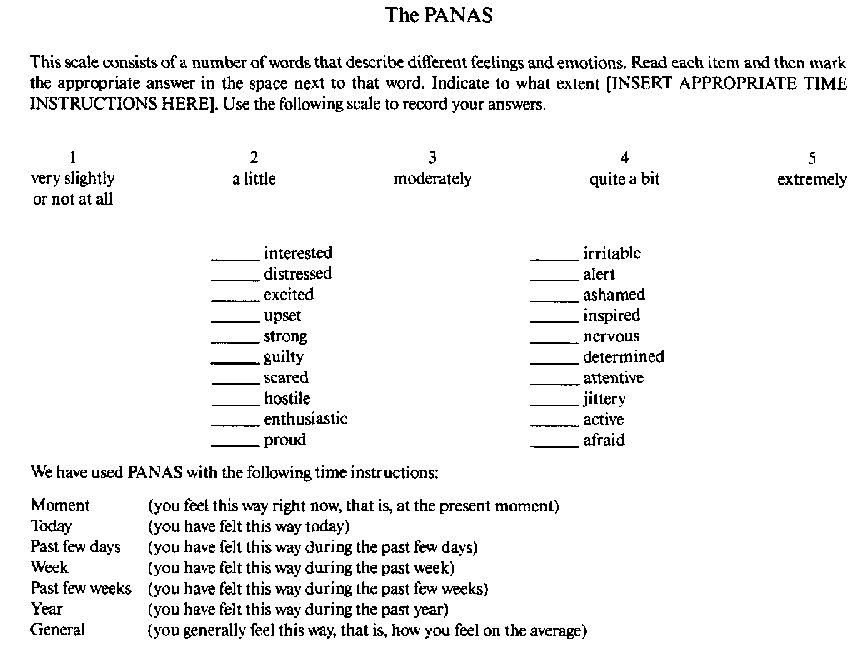
\includegraphics[width=\textwidth]{panas}
	
\end{frame}}

{\aauwavesbg%
	\begin{frame}{Stemningsregistrering} % the plain option removes the sidebar and header from the title page
		Patienten reflekterer over sit eget stemningsleje
		
		\begin{center}
		\begin{tabular}{|c|}
			\hline \cellcolor{red} Svær mani \\ 
			\hline \cellcolor{red!60} Moderat mani \\ 
			\hline \cellcolor{red!20} Let mani \\ 
			\hline \cellcolor{yellow} Normal \\ 
			\hline \cellcolor{blue!20} Let mani \\ 
			\hline \cellcolor{blue!60} Moderat mani \\ 
			\hline \cellcolor{blue} Svær mani \\ 
			\hline 
		\end{tabular} 
		\end{center}
	\end{frame}}
	
{\aauwavesbg%
	\begin{frame}{Stemningsregistrering} % the plain option removes the sidebar and header from the title page

		Angst specificeres på følgende skala:
		\begin{tabular}{| c | l|}
			\hline 0 & Ingen angst \\ 
			\hline 1 & lettere angst der ikke påvirker hverdagen\\ 
			\hline 2 & Konstant angst, funktionsniveau påvirkes\\ 
			\hline 3 & Udtalt angst, kan næsten ikke foretage sig noget\\
			\hline
		\end{tabular} 
	\end{frame}}
	
{\aauwavesbg%
	\begin{frame}{Stemningsregistrering} % the plain option removes the sidebar and header from the title page
		
		Derudover noteres detaljer om patientens hverdag
		\begin{itemize}
			\item Antal timers søvn
			\item Medicinforbrug
			\item Vægt
			\item Menstruation
		\end{itemize}
	\end{frame}}
	
{\aauwavesbg%
\begin{frame}{HAM-D} % the plain option removes the sidebar and header from the title page
	\begin{itemize}
		\item En mængde faktorer besvares givet mellem 3 og 5 svarmuligheder
		\item Score beregnes
		\item Stemningsleje vurderes
	\end{itemize}
	
\end{frame}}
	
{\aauwavesbg%
	\begin{frame}{Eksempler på spørgsmål} % the plain option removes the sidebar and header from the title page
		 Arbejde og interesser
		\begin{itemize}
			\item Ingen problemer
			\item Været mindre interesseret i de daglige aktiviteter eller følt sig lidt besværet
			\item Har følt sig noget insufficient i sine daglige aktiviteter
			\item Har haft svært ved at udføre selv de mere rutineprægede aktiviteter
			\item Har ikke været i stand til at udføre de rutineprægede aktiviteter uden hjælp
		\end{itemize}
		
	\end{frame}}

\subsection{Behov}
{\aauwavesbg%
\begin{frame}{Behov} % the plain option removes the sidebar and header from the title page
For at kunne udføre de tre nævnte metoder skal vi kunne stille følgende typer af spørgsmål


\begin{itemize}
	\item Angivelse af værdi på Likert-skala
	\item Fri tekst
	\item Valg mellem tekstuelle predefinerede svarmuligheder
	\begin{itemize}
		\item Skal kunne tillægges farver
	\end{itemize}
\end{itemize}
\end{frame}}

\subsection{Demonstration}
{\aauwavesbg%
\begin{frame}{Demonstration af implementeret modul} % the plain option removes the sidebar and header from the title page
	Det implementerede modul består af følgende:
	\begin{itemize}
		\item Scheduler
		\item Notifikationer
		\item Spørgsmål
	\end{itemize}
\end{frame}}


% includes her

\bgroup
\setbeamercolor{background canvas}{bg=black}
\begin{frame}[plain]{}
\addtocounter{framenumber}{-1}	
	\begin{center}
	%\textcolor{white}{END}
	\end{center}
\end{frame}
\egroup
	
\end{document}
